\documentclass[mathserif]{beamer}
\usetheme[secheader]{pecostalk}
\graphicspath{{figs/}}                                                                                                                              

\newcommand{\eqdef}{\stackrel{\text{\tiny def}}{=}}

\newcommand{\NVRvect}[1]{\ensuremath\boldsymbol{#1}}
\newcommand{\NVRtensor}[1]{\underline{\NVRvect{#1}}}
\newcommand{\NVRnorm}[1]{\left|\left|#1\right|\right|}
\newcommand{\NVRgrad}{\nabla}
\newcommand{\NVRdiv}{\NVRgrad \cdot}
\newcommand{\NVRpd}[2]{\frac{\partial#1}{\partial#2}}
\newcommand{\NVRpdd}[2]{\frac{\partial^2#1}{\partial#2^2}}
\newcommand{\NVReqdef}{\stackrel{\text{\tiny def}}{=}}

\newcommand{\NVRHgrad}{H(\text{grad})}
\newcommand{\NVRHdiv}{H(\text{div})}
\newcommand{\NVRsumm}[2]{\ensuremath\displaystyle\sum\limits_{#1}^{#2}}

\date{March 2-3, 2012}
\author{Nate Roberts}
\institute{The University of Texas at Austin}
\title[Camellia]{Camellia}
\subtitle{A Discontinuous Petrov-Galerkin Toolbox Using Trilinos}

\begin{document}
\begin{frame}
\begin{center}

\includegraphics[width=.8\linewidth]{grand_logo}\\
\end{center}
\titlepage
\begin{flushright}

\includegraphics[scale=0.1]{asc_logo}\\
\end{flushright}
\end{frame}

%===============================================================================
% ACKNOWLEDGEMENTS
%===============================================================================
\begin{frame}
\frametitle{Acknowledgments}

Collaborators:
\begin{itemize}
\item Leszek Demkowicz (UT/PECOS)
\item Denis Ridzal (Sandia/CSRI)
\item Pavel Bochev (Sandia/CSRI)
\item Jesse Chan (UT/PECOS)
\end{itemize}

Support:
\begin{itemize}
\item Sandia (summer internships)
\item PECOS (GRA funding)
\item ICES (CSEM Fellowship)
\end{itemize}

\end{frame}


%===============================================================================
% OUTLINE
%===============================================================================
\begin{frame}
\frametitle{Outline}

\begin{enumerate}
\item DPG Intro
\item Goals for Camellia
\item Selected Design Ideas within Camellia
\item A Performance Issue, and its Resolution
\item Current and Future Work
\end{enumerate}

\end{frame}

%===============================================================================
% From Strong-Form PDE to DPG Form
%===============================================================================
\begin{frame}                                                                                                                                                                          
\frametitle{From Strong-Form PDE to DPG Form}
\begin{center}
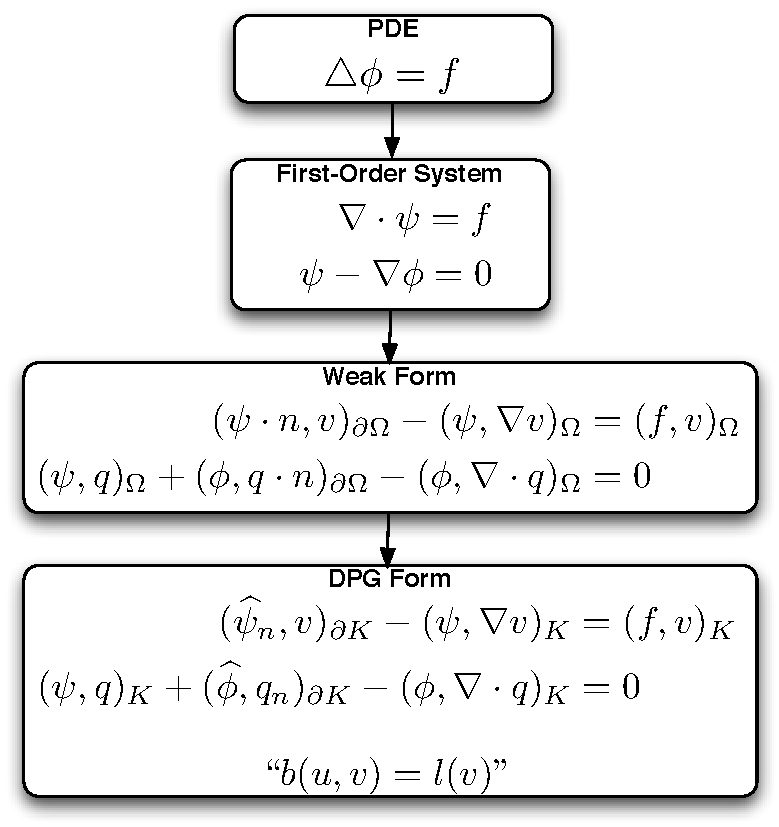
\includegraphics[width=.6\linewidth]{DPGFormCartoon}\\
\end{center}
\end{frame}              
%===============================================================================
% Solving with DPG
%===============================================================================
\begin{frame}                                                                                                                                                                          
\frametitle{Solving with DPG}
\begin{center}
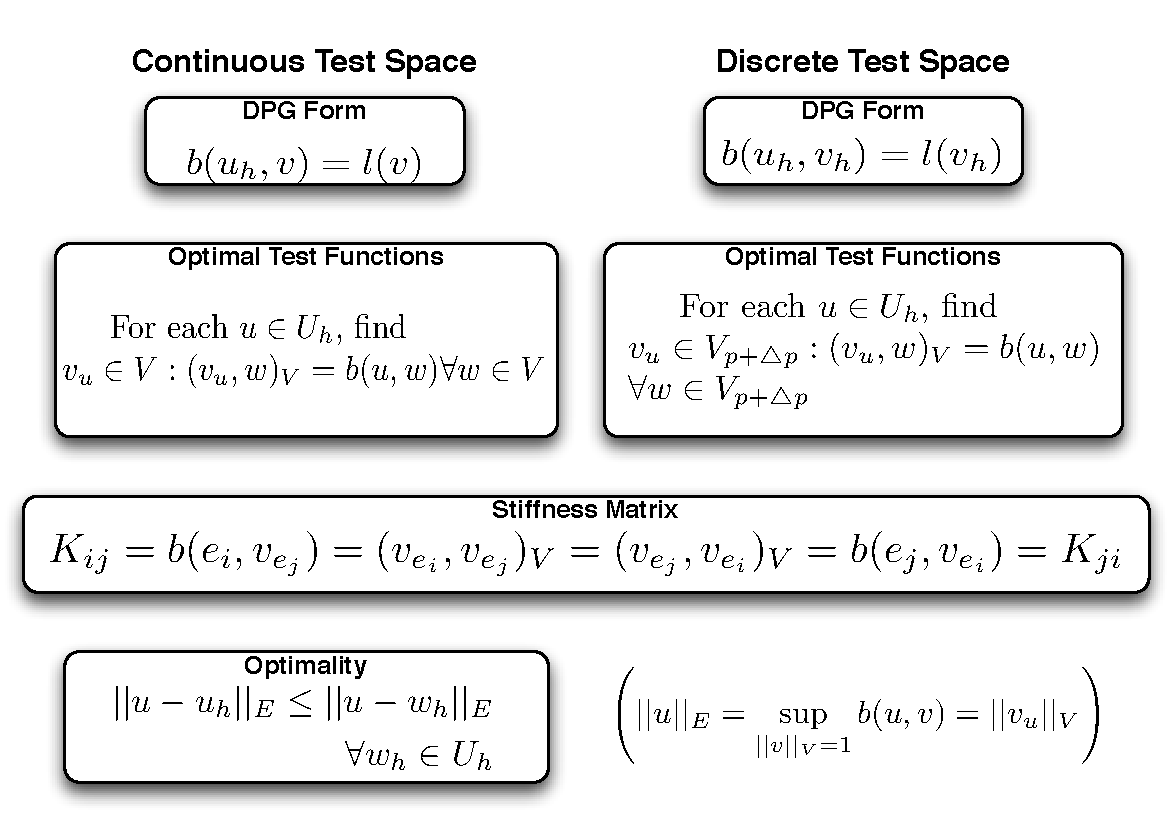
\includegraphics[width=0.9\linewidth]{DPGSolveCartoon}\\
\end{center}
\end{frame}

%===============================================================================
% CAMELLIA GOALS
%===============================================================================
\begin{frame}
\frametitle{Goals for Camellia}
\begin{block}{Goals for Camellia (Achieved)}
\begin{itemize}
\item Define $b(u,v)$ in the \emph{continuous} space (separation of concerns)
\item Arbitrary, hp-adaptive 2D meshes (quads and triangles)
\item ``Reasonable'' speed and scalability
\item Provide prebuilt versions of inner products commonly used in DPG research (mathematician's and quasi-optimal)
\end{itemize}
\end{block}

\vspace{3 mm}

\begin{block}{Goals for Camellia (Aspirational)}
\begin{itemize}
\item Support for nonlinear PDEs (Navier-Stokes in particular)
\item Better scalability
\item Longer term: 3D meshes
\end{itemize}
\end{block}

\end{frame}


%===============================================================================
% WHAT INTREPID (TRILINOS) PROVIDES
%===============================================================================
\begin{frame}
\frametitle{Trilinos Support}
\begin{block}{Provided by Intrepid}
\begin{itemize}
\item Conforming basis functions 
\item Basis value transformations from reference to physical space
\item Numerical integration facilities
\end{itemize}
\end{block}

The Intrepid facilities operate on \emph{batches} of like elements.

\vspace{3 mm}

\begin{block}{Provided by Epetra}
\begin{itemize}
\item Distributed storage types (including Epetra::FECrsMatrix)
\item Abstract linear solver interfaces (easy to switch solvers)
\end{itemize}
\end{block}

\end{frame}

%===============================================================================
% ELEMENT TYPE
%===============================================================================
\begin{frame}
\frametitle{Design Idea: Element Type}

\begin{center}
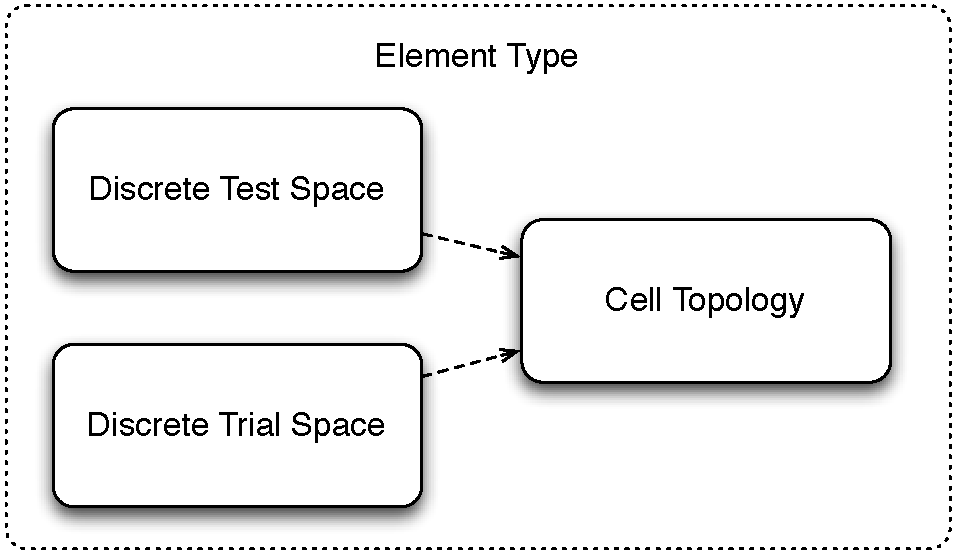
\includegraphics[width=8.5cm]{ElementType}
\end{center}

To take maximal advantage of Intrepid's support for batches of elements while operating on a non-uniform mesh,
we introduce the notion of the element type.  Elements of the same type agree in terms of their discrete test and trial spaces.

\end{frame}


%===============================================================================
% ELEMENT TYPE
%===============================================================================
\begin{frame}
\frametitle{Design Idea: Discrete Space}

\begin{center}
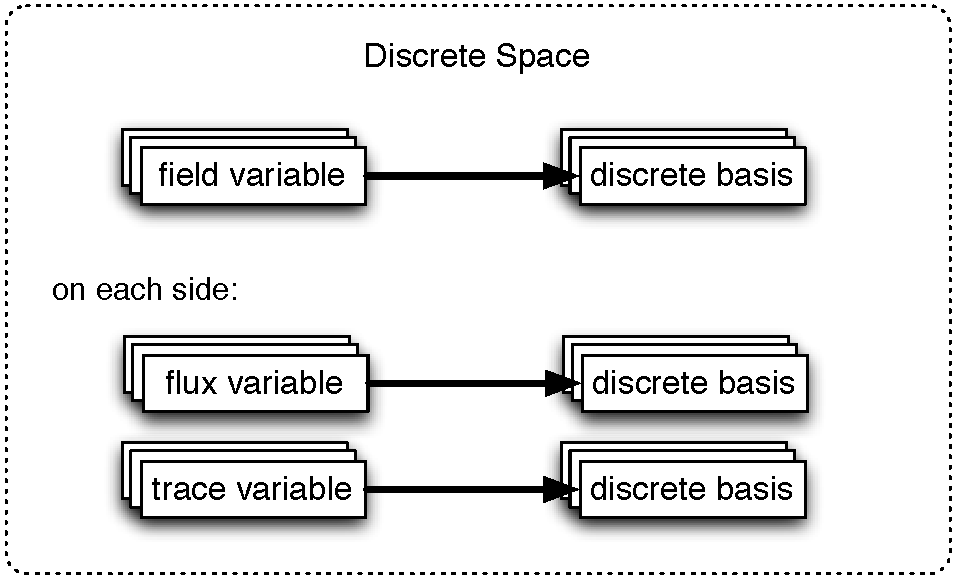
\includegraphics[width=8.5cm]{DiscreteSpace}
\end{center}

The discrete spaces, in turn, are defined by mappings from variables to the bases used to represent them.

\end{frame}

%===============================================================================
% FACTORY DESIGN PATTERN
%===============================================================================
\begin{frame}
\frametitle{Design Pattern: Factory}

Each element has a type; each type has a pair of discrete spaces; each discrete space is made up of several bases.  How do we keep this design from taking a prohibitive amount of memory?\\
\vspace{3 mm}
For this, among other considerations: want a way to guarantee that we only create one copy of each basis, discrete
space, and element type.  This is known as a \emph{Factory} in the design pattern literature.

\begin{block}{Create Factories for:}
\begin{itemize}
\item Basis
\item Discrete Space
\item Element Type
\end{itemize}
\end{block}

\end{frame}

%===============================================================================
% PERFORMANCE ISSUES
%===============================================================================
\begin{frame}
\frametitle{Performance Story: Quasi-Optimal Inner Product}

The ``optimal test norm''---a choice of test space norm that deliver best approximation in $||\cdot||_{U}$---is given by 
\begin{align*}
||v||_{V}\eqdef \sup_{||u||_{U}=1} b(u,v).
\end{align*}
\\
\begin{itemize}
\item When $U=L^{2}$, can determine analytically using Cauchy-Schwarz.
\item Approximate with ``localized'' version, the \emph{quasi-optimal} test norm.
\item Camellia can determine quasi-optimal test norm automatically.
\end{itemize}

However, when I first implemented this and used it in place of the ``mathematician's'' norm, I observed a dramatic reduction in overall speed.  Why?

\end{frame}


\begin{frame}
\frametitle{Performance Story: Quasi-Optimal Inner Product}

The mathematician's norm for my Stokes formulation is:
\begin{align*}
\NVRnorm{(\NVRvect{q}_{1},\NVRvect{q}_{2},v_{1},v_{2},v_{3})}_{V}^{2}  \NVReqdef \NVRsumm{i=1}{2} ||\NVRvect{q}_{i}||_{\NVRHdiv}^{2} + \NVRsumm{i=1}{3} ||v_{i}||_{\NVRHgrad}^{2} \label{NVR:eq:genericNorm}\\
\end{align*}

Compare the quasi-optimal test norm:
\begin{align*}
& \NVRnorm{\frac{q_{11}}{2\mu}+\NVRpd{}{x}v_{1}}_{L^2}^{2} + \NVRnorm{\frac{q_{11}}{2\mu}+\frac{q_{22}}{2\mu}}_{L^2}^{2} + \NVRnorm{\frac{q_{12}}{2\mu}+\frac{q_{21}}{2\mu}+\NVRpd{}{y}v_{1}+\NVRpd{}{x}v_{2}}_{L^2}^{2}\\
&\left. + \NVRnorm{\frac{q_{22}}{2\mu}+\NVRpd{}{y}v_{2}}_{L^2}^{2} + \NVRnorm{q_{12}-q_{21}}_{L^2}^{2} + \NVRnorm{\NVRdiv \NVRvect{q}_{1}-\NVRpd{}{x}v_{3}}_{L^2}^{2} \right.\\
&+\NVRsumm{i=1}{2} ||\NVRvect{q}_{i}||_{L^{2}}^{2} + \NVRsumm{i=1}{3} ||v_{i}||_{L^{2}}^{2}\\
\end{align*}

\end{frame}


\begin{frame}
\frametitle{Design Idea: BasisCache}

\begin{itemize}
\item Discrete spaces $\implies$ quadrature points.
\item Will use each basis repeatedly---especially in quasi-optimal test norm!---in both reference and physical space.
\end{itemize}

\begin{itemize}
\item Procedural idea: compute these values once, store them, and reuse them.
\item Object-oriented analog: a cache of basis values (lazily computed, with a limited lifespan).
\item Core computational components---BilinearForm, RHS, and InnerProduct---take a BasisCache as an argument.
\end{itemize}

Once implemented, the quasi-optimal test norm was nearly as fast as the mathematician's norm...

\end{frame}

%===============================================================================
% CURRENT AND FUTURE WORK
%===============================================================================
\begin{frame}
\frametitle{Current and Future Work}
\begin{block}{}
\begin{itemize}
\item Nonlinear PDE support
\item Better scalability (distributed mesh)
\item Application to Navier-Stokes
\end{itemize}
\end{block}

\begin{columns}[c]
\begin{column}{5.5cm}
\begin{block}{Convection-Diffusion, $\epsilon=10^{-2}$}
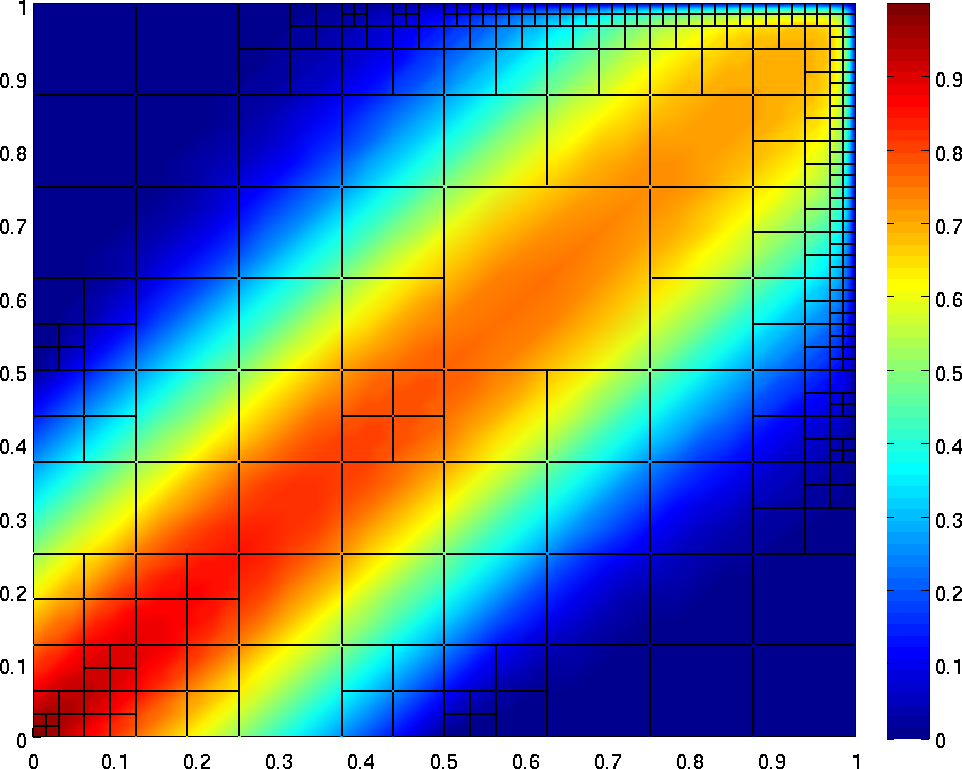
\includegraphics[width=5.5cm]{confusionDemo.png}
\end{block}
\end{column}
\begin{column}{5.5cm}
\begin{block}{Burgers', $\epsilon=10^{-4}$}
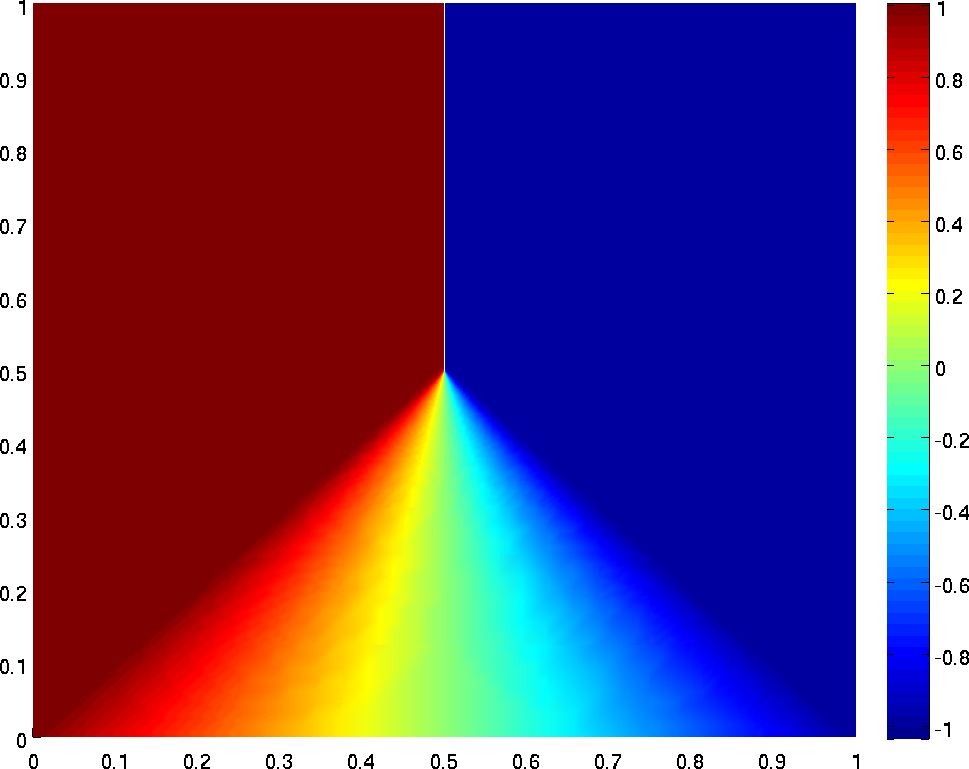
\includegraphics[width=5.5cm]{burgers1e4.png}
\end{block}
\end{column}
\end{columns}
\end{frame}


%===============================================================================
% NEW SLIDE
%===============================================================================
\begin{frame}
\frametitle{}
\begin{block}{}
\center{Thank you!} \\
\center{Questions?}\\
%For more info:\\
%nroberts@ices.utexas.edu\\
%\url{https://cfwebprod.sandia.gov/cfdocs/CCIM/docs/Roberts_et_al_SAND2011-6678.pdf}
\end{block}

\end{frame}

 
\end{document}
